\documentclass[xcolor={dvipsnames}]{beamer}
\usepackage{import}
\import{C:/Users/ryanj/Dropbox/code/LatexMacros/}{mymacros2.tex}

\usetheme{metropolis}
\usecolortheme[snowy]{owl}


\title{ Week 7 Discussion Section Questions}
\author{Ryan Martin}


\begin{document}


	\begin{frame}{Table of Contents}
		\tableofcontents
	\end{frame}

	\section{Question 1}

		
	\begin{frame}[allowframebreaks]{Scratch}
	$p_{2^s} + \U(1^s, \upsilon) - \U(2^s, \upsilon)$
	
	$p_{1^e}^f + \U(1^s, \upsilon) - \U(1^e, \upsilon)$
	
	$p_{1^s}^0 + \U(1^e, \upsilon) - \U(1^s, \upsilon)$
	
	
	$S^{CV}=-\int_{p_{1^e}^f}^\infty \1\set{\U(1^e, \upsilon) - p > \U(1^s, \upsilon) - p_{1^s}^0}dp$
	
	$p_{1^s}^0$
	
	$p_{1^e}^f$
	$Q^{1^e}$
	$Q^{1^s}$
	$-S^{CV}$
	
	Demand for Good $1^s$ When $1^s$ Preferred \\
	Demand for Good $1^e$ When $1^e$ Preferred \\
	
	
	
	$Q_1(p_1)$
	
	$Q_2(p_1)$
	
	$Q$
	
	$P$
	
	$Q_1$
	
	$Q_2$
	
	
	
	Shift
	\end{frame}


\begin{frame}[allowframebreaks]
	$p_{D^1}^1 + \tilde{U}_{D^0}(\eta) - \tilde{U}_{D^1}(\eta)$
	$\bar{p}$ s.t. $U_{D^0}(y - \bar{p}, \eta) = U_{D^1}(y - p_{D^1}^1, \eta)$
	Demand for Good $D^0$ When $D^0$ Preferred to $D^1$
	
	\end{frame}
	
	\begin{frame}[allowframebreaks]{6.3}
	Consider the model $$y = \beta_1 + x_2 \beta_2 + x_3 \beta_3 + e$$ and suppose that application of least squares to 20 observations on these variables yields the following results $$\begin{bmatrix}
		b_1 \\
		b_2 \\
		b_3
	\end{bmatrix}  = \begin{bmatrix} .96587 \\ .69914 \\ 1.7769 \end{bmatrix}$$ and $$\widehat{cov(b)} = \begin{bmatrix} .21812 & .019195 & -.050301 \\ .019195 & .048526 & -.031223 \\ -.050301 & -.031223  & .037120 \end{bmatrix} $$ with $$\hat{\sigma}^2 = 2.5193, \hspace*{1cm} R^2 = .9466$$
	
	\begin{itemize}
		\item[a] Find the total variation, unexplained variation and explained variation for this model
		
		
		\item[b] Find 95\% interval estimates for $\beta_2$ and $\beta_3$.
		
		\item[c] Use a t-test to test the hypothesis $H_0: \beta_2 \ge 1$ against the alternative $H_1: \beta_2 < 1$
		
		
		\item[d] Use your answers in part (a) to test the joint hypothesis $H_0: \beta_2 = 0, \beta_3 = 0$.
		
		\item[e] Test the hypothesis $H_0: 2 \beta_2 = \beta_3$  
		
	\end{itemize}
	
\end{frame}
	
	
	\section{Question 2}
	
	\begin{frame}[allowframebreaks]{6.4}
	\textit{This was a homework problem, but I solved it too}
	
	Consider the wage equation 
	\begin{align*}
	\log(WAGE) & = \beta_1 + \beta_2 EDUC + \beta_3 EDUC^2 + \beta_4 EXPER + \beta_5 EXPER^2\\
	& \hspace*{1cm} + \beta_6 (EDUC \times EXPER) + \beta_7 HRSWK + e
	\end{align*}
	 where the explanatory variables are years of education, years of experience and hours worked per week. Estimation results for this equation, and for modified versions of it obtained by dropping some of the variables, are displayed in Table 6.4. These results are from the 1000 observations in the file \texttt{cps4c\_small.dat}
	
	\begin{itemize}
		\item[a] Using an approximate 5\% critical value of $t_c = 2$, what coefficient estimates are not significantly different form zero?
		
		
		
		
		\item[b] What restriction on the coefficients of Eqn (A) gives Eqn(B)? Use an F-test to test this restriction. Show how the same result can be obtained using a t-test.
		
		\item[c] What restrictions on the coefficients of Eqn (A) gives Eqn(C)? Use an F-test to test these restrictions. What question would you be trying to answer by performing this test?
		
		\item[d] What restrictions on the coefficients of Eqn (B) give Eqn (D)? Use an F-test to test these restrictions. What question would you be trying to answer by performing this test?
		 
		\item[e] What restrictions on the coefficients of Eqn (A) give Eqn (E)? Use an F-test to test these restrictions. What question would you be trying to answer by performing this test?
		
		\item[f] Based on your answers to parts (a) to (e), which model would you prefer? Why?
		
		\item[g] Compute the missing AIC value for Eqn (D) and the missing SC value for Eqn (A). Which model is favored by the AIC? Which model is favored by the SC?
	\end{itemize}
	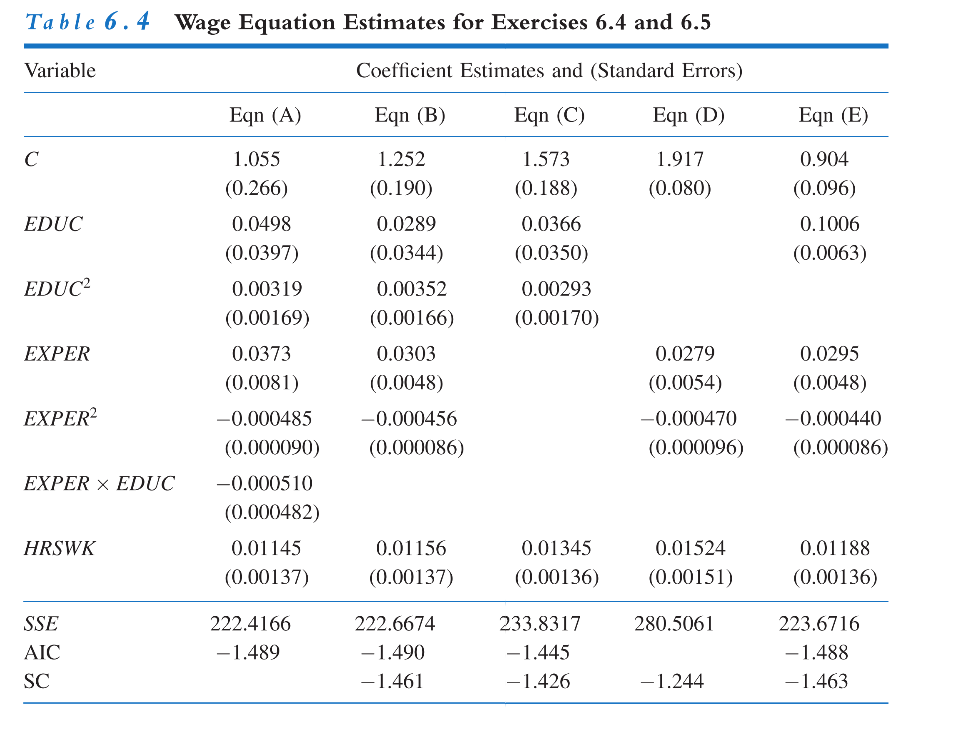
\includegraphics{Table6_4.png}
	
\end{frame}


	\section{Question 3}
\begin{frame}[allowframebreaks]{6.14}
	Following on from the example in section 6.3, the file hwage.dat contains another subset of the data used by labor economist Tom Mroz. The variables with which we are concerned are \begin{itemize} 
		\item HW - Husband's wage in 2006 dollars
		\item HE - Husband's education attainment in years
		\item HA - Husband's age
		\item CIT - a variable equal to one if living in a large city, otherwise zero.
		\end{itemize}
	
	\begin{itemize}
		\item[a] Estimate the model $$HW = \beta_1 + \beta_2 HE + \beta_3HA + e$$ What effects do changes in the level of education and age have on wages?
	

	\item[b] Does RESET suggest that the model in part (a) is adequate?
	
	\item[c] Add the variables $HE^2$ and $HA^2$ to the original equation and re-estimate it. Describe the effect that education and age have on wages in this newly estimated model. 
	
	\item[d] Does RESET suggest that the model in part (c) is adequate?
	\item[e] Reestimate the model in part(c) with the variable CIT included. What can you say about the level of wages in large cities relative to outside those cities?
	
	\item[f] Do you think $CIT$ should be included in the equation?
	
	\item[g] For both the model estimated in part (c) and the model estimated in part (e) evaluate the following four derivatives:
	
	\begin{itemize}
		\item $\frac{\partial HW}{\partial HE} $ for $HE = 6$ and $HE = 15$
		\item $\frac{\partial HW}{\partial HA} $ for $HA = 35$ and $HA = 50$
	\end{itemize}
Does the omission of CIT lead to omitted-variable bias? Can you suggest why?
\end{itemize}

\end{frame}

\section{6.22}
\begin{frame}[allowframebreaks]{6.22}
6.22

In Chapter 5.7 we used the data in file pizza4.dat to estimate the model $$PIZZA = \beta_1 + \beta_2 AGE + \beta_3 INCOME + \beta_4 (AGE \times INCOME) + e$$

\begin{itemize}
	\item[a]
Test the hypothesis that age does not affect pizza expenditure - that is, test the joint hypothesis $H_0 \beta_2 = 0, \beta_4 = 0$. What do you conclude?

\item[b]
Construct point estimates and .95 CI for the marginal propensity to spend on pizza for individuals of ages 20, 30, 40, 50 and 55. Comment on these estimates.

\item[c]
Modify the equation to permit a "life-cycle" effect in which the marginal effect of income on pizza expenditure increases with age, up to a point, then falls. Do so by adding the term $(AGE^2 \times INC)$ to the model. What sign do you anticipate on this term? Estimate the model and test the significance of the coefficient for this variable. Did the estimate have the expected sign?

\item[d]
Using the model in (c) e marginal propensity to spend on pizza for individuals of ages 20, 30, 40, 50 and 55. Comment on these estimates. In light of these values and of the range of the age in the sample data, what can you say about the quadratic function of age that describes the marginal propensity to spend on pizza?

\item[e]
For the model in part (c), are each of the coefficient estimates for AGE $(AGE \times INC)$ and $(AGE^2 \times INC)$ significantly different from 0 at a 5\% level? Carry out a joint test for the significance of these variables. Comment on your results.

\item[f]
Check the model used in part (c) for collinearity. Add the term ($AGE^3 \times INC$) to the model in (c) and check the resulting model for collinearity.

\end{itemize}

\end{frame}



\end{document}
